\documentclass[main.tex,fontsize=8pt,paper=a4,paper=portrait,DIV=calc,]{scrartcl}
% Document
\usepackage[T1]{fontenc}
\usepackage[utf8]{inputenc}
\usepackage[dvipsnames]{xcolor}
\usepackage[nswissgerman,english]{babel} 
\usepackage{hyperref}
\renewcommand{\familydefault}{\sfdefault}

% Format
\usepackage[top=5mm,bottom=1mm,left=5mm,right=5mm]{geometry}
%\setlength{\headheight}{\baselineskip}
%\setlength{\headsep}{0mm}

%\usepackage{scrlayer-scrpage}
%\clearpairofpagestyles
%\chead{{\bfseries\TITLE, \AUTHOR, \pagename~\thepage}}

%\addtokomafont{pagehead}{\upshape}

\usepackage{multicol}
\setlength{\columnsep}{2mm}
\setlength{\columnseprule}{0.1pt}

% Math
\usepackage{amsmath}
\usepackage{amssymb}
\usepackage{amsfonts}

% Code
\usepackage{fancyvrb, etoolbox, listings, xcolor}
%\usemintedstyle{bw}

%\newminted[shell]{bash}{
%fontsize=\footnotesize,
%fontfamily=tt,
%breaklines=true,
%frame=single,
%framerule=0.1pt,
%framesep=2mm,
%tabsize=2
%}
%\newminted{css}{
%breaklines=true,
%tabsize=4,
%autogobble=true,
%escapeinside=||,
%stripall=true,
%stripnl=true,
%}

    \definecolor{lightgray}{rgb}{0.95, 0.95, 0.95}
    \definecolor{darkgray}{rgb}{0.4, 0.4, 0.4}
    \definecolor{purple}{rgb}{0.65, 0.12, 0.82}
    \definecolor{ocherCode}{rgb}{1, 0.5, 0} % #FF7F00 -> rgb(239, 169, 0)
    \definecolor{blueCode}{rgb}{0, 0, 0.93} % #0000EE -> rgb(0, 0, 238)
    \definecolor{greenCode}{rgb}{0, 0.6, 0} % #009900 -> rgb(0, 153, 0)
    \definecolor{teal}{rgb}{0.0, 0.5, 0.5}

\lstdefinestyle{code}{
    identifierstyle=\color{black},
    keywordstyle=\color{blue}\bfseries\small,
    ndkeywordstyle=\color{greenCode}\bfseries\small,
    stringstyle=\color{ocherCode}\ttfamily\small,
    commentstyle=\color{teal}\ttfamily\textit\small,
    basicstyle=\ttfamily\small,
    breakatwhitespace=false,         
    breaklines=true,                 
    captionpos=b,                    
    keepspaces=true,                 
    showspaces=false,                
    showstringspaces=false,
    showtabs=false,                  
    tabsize=2,
    belowskip=-5pt
}



% Images
\usepackage{graphicx}
\newcommand{\pic}{\includegraphics[scale=0.3]}
\graphicspath{{Screenshots/}{../Screenshots}}
\makeatletter
\def\pictext#1#2{%
    \@ifnextchar[{%
    \pictext@iiiii{#1}{#2}%
    }{%
      \pictext@iiiii{#1}{#2}[0.5,0.4,0.3]% Default is 5
    }%
}
\def\pictext@iiiii#1#2[#3,#4,#5]{\begin{minipage}{#3\textwidth}\includegraphics[scale=#4]{#1}\end{minipage}\begin{minipage}{#5\textwidth}#2\end{minipage}}
\def\minipg#1#2{%
    \@ifnextchar[{%
    \minipg@iiii{#1}{#2}%
    }{%
      \minipg@iiii{#1}{#2}[0.3,0.6]% Default is 5
    }%
}
\def\minipg@iiii#1#2[#3,#4]{\vspace{0.8mm}\begin{minipage}{#3\textwidth}#1\end{minipage}\begin{minipage}{#4\textwidth}#2\end{minipage}{\vspace{0.8mm}}}
\makeatother

%\newenvironment{minty}[2]% environment name
%{% begin code
%  \begin{minipage}{#1}
%  \begin{minted}{#2}
%}%
%{% end code
%  \end{minted}
%  \end{minipage}
%  \end{minty}\ignorespacesafterend
%} 

% Smaller Lists
\usepackage{enumitem}
\setlist[itemize,enumerate]{leftmargin=3mm, labelindent=0mm, labelwidth=1mm, labelsep=1mm, nosep}
\setlist[description]{leftmargin=0mm, nosep}
\setlength{\parindent}{0cm}

% Smaller Titles
\usepackage[explicit]{titlesec}

%% Color Boxes
\newcommand{\sectioncolor}[1]{\colorbox{black!60}{\parbox{0.989\linewidth}{\color{white}#1}}}
\newcommand{\subsectioncolor}[1]{\colorbox{black!50}{\parbox{0.989\linewidth}{\color{white}#1}}}
\newcommand{\subsubsectioncolor}[1]{\colorbox{black!40}{\parbox{0.989\linewidth}{\color{white}#1}}}
\newcommand{\paragraphcolor}[1]{\colorbox{black!30}{\parbox{0.989\linewidth}{\color{white}#1}}}
\newcommand{\subparagraphcolor}[1]{\colorbox{black!20}{\parbox{0.989\linewidth}{\color{white}#1}}}

%% Title Format
\titleformat{\section}{\vspace{0.5mm}\bfseries}{}{0mm}{\sectioncolor{\thesection~#1}}[{\vspace{0.5mm}}]
\titleformat{\subsection}{\vspace{0.5mm}\bfseries}{}{0mm}{\subsectioncolor{\thesubsection~#1}}[{\vspace{0.5mm}}]
\titleformat{\subsubsection}{\vspace{0.5mm}\bfseries}{}{0mm}{\subsubsectioncolor{\thesubsubsection~#1}}[{\vspace{0.5mm}}]
\titleformat{\paragraph}{\vspace{0.5mm}\bfseries}{}{0mm}{\paragraphcolor{\theparagraph~#1}}[{\vspace{0.5mm}}]
\titleformat{\subparagraph}{\vspace{0.5mm}\bfseries}{}{0mm}{\subparagraphcolor{\thesubparagraph~#1}}[{\vspace{0.5mm}}]

%% Title Spacing
\titlespacing{\section}{0mm}{0mm}{0mm}
\titlespacing{\subsection}{0mm}{0mm}{0mm}
\titlespacing{\subsubsection}{0mm}{0mm}{0mm}
\titlespacing{\paragraph}{0mm}{0mm}{0mm}
\titlespacing{\subparagraph}{0mm}{0mm}{0mm}

%% format cells
\usepackage[document]{ragged2e}
\usepackage{array, makecell}
\renewcommand{\arraystretch}{2}
\newcommand{\mc}{\makecell[{{m{1\linewidth}}}]}



\allsectionsfont{\centering}
\begin{document}
\centering
\tableofcontents

\lstset{
    language=Java,
    style=code,
}

\newcommand{\TITLE}{Parallel Programming}
\newcommand{\AUTHOR}{Fabio Lenherr}
\setcounter{tocdepth}{1}

\section{Motivation}

\subsection{Moore's Law}
Until now the idea was that more transistors, more GHz, etc means that we can go faster and faster.
However, the issue is that the increases are getting slower and slower, while the workloads are getting increasingly complex with clear need for \emph{multithreading}.

\subsection{Hyperthreading vs Multiple Cores}
\minipg{
Hyperthreading creates the illusion of multiple cores via switching the context of the registers efficiently.\newline
In other words, it just properly streamlines computation similar to JS await/async.\newline
\textcolor{purple}{Note the different instruction set and the same compute core with hyperthreading!}
}{
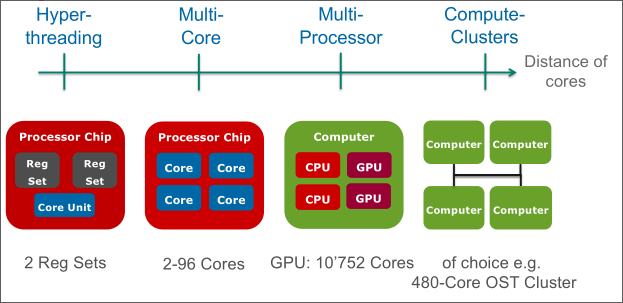
\includegraphics[scale=0.4]{2023_02_20_08_47_23.png}\newline
}[0.55,0.5]

\subsection{Concurrent vs Parallel}
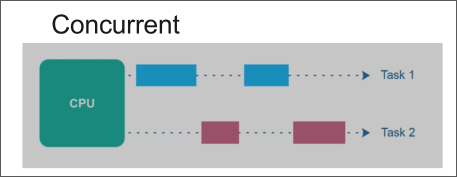
\includegraphics[scale=0.4]{2023_02_20_08_45_03.png}
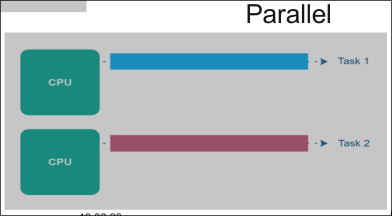
\includegraphics[scale=0.4]{2023_02_20_08_45_08.png}

\subsubsection{Concurrency}
Concurrency has the goal of \emph{simpler programs}, it does this by offering \emph{simultaneous or interleaved(time shared)} execution that accesses shared resources. 

\subsubsection{Parallelism}
Parallelism has the goal of \emph{faster programs}, it does this by decomposition of a program into \emph{several sub-programs}, which can run in parallel on multiple processors or cores.

\section{Parallel Programming in OS Space}

\subsection{Processes and threads}
\minipg{
A process is the instance of a program, while a thread is a subpart of a program, which will then have different callstacks. Meaning that each thread will have it's own callstack but share the same heap!
}{
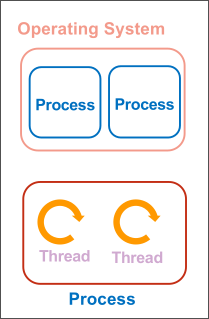
\includegraphics[scale=0.4]{2023_02_20_09_03_15.png}
}[0.7,0.3]\newline
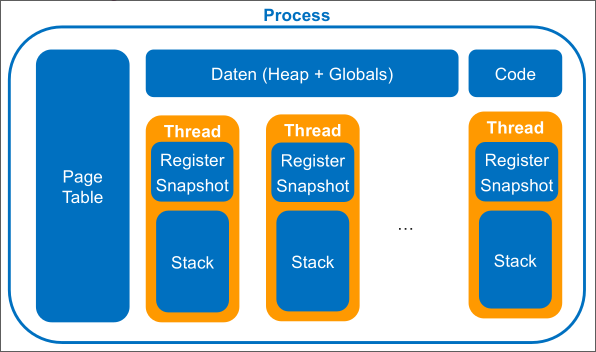
\includegraphics[scale=0.4]{2023_02_20_09_04_01.png}

\subsection{Pros and Cons}
\minipg{
  Cons:
\begin{itemize}
\item \textcolor{red}{Interprocess Communication}
\item \textcolor{red}{Process Management via system calls}
\item \textcolor{red}{Memory isolation}
\end{itemize} 
}{
  Pros:
  \begin{itemize}
  \item \textcolor{green}{Process isolation}
  \item \textcolor{green}{Responsiveness}
  \end{itemize} 
}[0.4,0.4]

\subsection{User threads vs Kernel threads}
\minipg{
  User level threads is a so-called \emph{green thread}, it can't offer true parallelism and is only scheduled by a runtime library or a virtual machine.
}{
  Kernel level thread is the true form of multithreading. \emph{native threads}\newline
It offers context switching via \emph{SW interrupt}.
}[0.25,0.25]

\subsection{Context Switch}
\begin{itemize}
\item \textcolor{purple}{Synchronous}
  \begin{itemize}
  \item \textcolor{black}{Thread waiting for condition}
  \item \textcolor{black}{queues itself as waiting and gives processor free}
  \item \textcolor{black}{locks processor during usage}
  \end{itemize} 
\item \textcolor{purple}{Asynchronous}
  \begin{itemize}
  \item \textcolor{black}{after some defined time the thread should release the processor}
  \item \textcolor{black}{prevent a thread from permanently occupying the processor (solves locks)}
  \end{itemize} 
\end{itemize} 

\subsection{Multi-Tasking}
\begin{itemize}
\item \textcolor{purple}{Cooperative}
  \begin{itemize}
  \item \textcolor{black}{threads must explicitly initiate context switches synchronously at the scheduler at intervals}
  \item \textcolor{black}{scheduler cannot interrupt running thread}
  \end{itemize} 
\item \textcolor{purple}{Preemptive}
  \begin{itemize}
  \item \textcolor{black}{scheduler can interrupt the running thread asynchronously via timer interrupt}
  \item \textcolor{black}{Time-Sliced scheduling: each thread has the processor for maximum time interval}
  \end{itemize} 
\end{itemize} 
\textcolor{red}{Preemptive is used for the most part!!}

\subsection{Thread States}
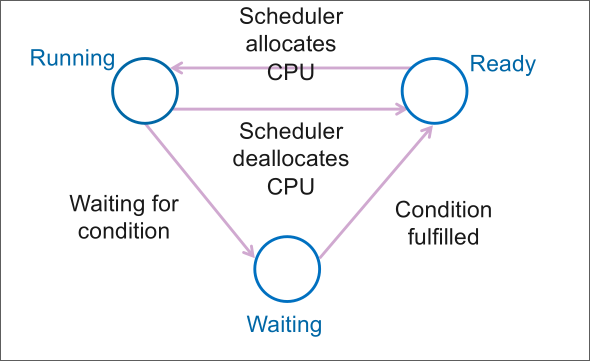
\includegraphics[scale=0.4]{2023_02_20_09_14_43.png}

\subsection{Non-determinism}
When using multi-threading, you can't be sure which thread will be used to complete a task first, meaning that if you print 2 different statements in 2 threads, then you can't be sure of the order in which these statements will be printed.

\section{Parallel Programming in Jafuck}
\subsection{Thread Implementation}
Java implements its own threads which are then linked to the kernel threads.\newline
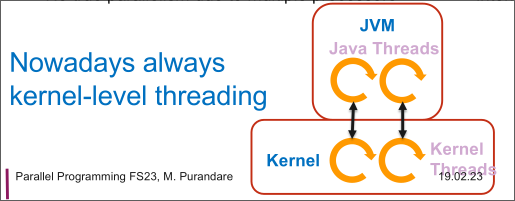
\includegraphics[scale=0.4]{2023_02_20_09_07_53.png}

\subsection{JVM Thread Model}
Java is a single process system -> JVM as one process on the operating system. \newline
\textcolor{purple}{JVM creates a thread at startup which calls main().}\newline
You are then free to call/create more threads as the programmer.

\subsection{JVM Termination}
\begin{itemize}
\item \textcolor{purple}{The JVM runs as long as threads are running, the main function doesn't matter in this case}\newline
  The only exception are so called \emph{daemon threads}, these are threads like the garbage collector, which ofc needs to be ignored for the jvm to EVER end.
\item \textcolor{purple}{You can exit manually via System.exit() or Runtime.exit()}\newline
  Note that this means uncontrolled termination of all threads.
  This can lead to \emph{undefined behavior}.
\end{itemize} 

\subsection{Thread in Java}
A thread in java takes a so called "runnable target", this is an interface that simply defines the type of behavior that can be run inside of a thread. \newline
For example the thread might run something like a lambda.
\begin{lstlisting}
public class Thread implements Runnable {
  private Runnable target;
  public synchronized void start() {
    if (threadStatus != 0)
      throw new IllegalThreadStateException();
    group.add(this);
    boolean started = false;
  }
  public void run() {
    if (target != null) {
      target.run(); 
    }
  }
  public Thread() {
    this(null, null, "Thread-" + nextThreadNum(), 0);
  }
  public Thread(Runnable target) {
    this(null, target, "Thread-" + nextThreadNum(), 0);
  }
}
\end{lstlisting}
\vspace{2mm}
\textcolor{purple}{Note that should a thread cause an exception, the other threads will continue to run!}

\subsection{Example for multithreading in java}
\begin{lstlisting}
public class MultiThreadTest {
  public static void main(String[] args) {
    var a = new Thread(() -> multiPrint("A"));
    var b = new Thread(() -> multiPrint("B"));
    a.start();
    b.start();
    System.out.println("main finished");
  }
  static void multiPrint(String label) {
    for (int i = 0; i < 10; i++) {
      System.out.println(label + ": " + i);
    }
  }
}
\end{lstlisting}
\vspace{2mm}
\textcolor{purple}{Lambdas as well as method references implement the runnable interface}

\subsection{Explicit/Sub-class Thread behavior}
You can explicitly set the behavior of a thread via overriding the run method of the runnable interface.\newline
Note that this means you will implement your own thread!\newline
\begin{lstlisting}
class SimpleLogic implements Runnable {
  @Override
  public void run() {
    // thread behavior
  }
}
var myThread = new Thread(new SimpleLogic());
myThread.start();
\end{lstlisting}
\vspace{2mm}
If you simply with to extend it you can extend the thread class instead:\newline
\begin{lstlisting}
class SimpleThread extends Thread {
  @Override
  public void run() {
    // thread behavior
  }
}
var myThread = new SimpleThread();
myThread.start();
\end{lstlisting}
\vspace{2mm}

\subsection{Thread join}
\minipg{
  This is used when you specifically want another thread to be blocked while another one is running, because you might have a usecase where that one thread needs to fulfill their job.
}{
  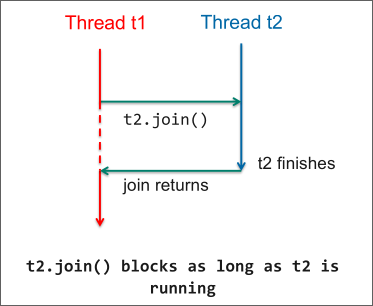
\includegraphics[scale=0.4]{2023_02_20_09_38_24.png}
}[0.6,0.4]
\begin{lstlisting}
var a = new Thread(() -> multiPrint("A"));
var b = new Thread(() -> multiPrint("B"));
System.out.println("Threads start");
a.start();
b.start();
a.join();
b.join();
System.out.println("Threads joined");
\end{lstlisting}
\vspace{2mm}

\subsection{Methods of a thread}
\begin{itemize}
\item \textcolor{purple}{thread.sleep(milliseconds)}\newline
  waits until time has elapsed before becoming ready again -> wait until it is scheduled again to run
\item \textcolor{purple}{thread.yield()}\newline
  thread releases processor and will be ready to be used again -> wait until it is scheduled again to run\newline
  \textcolor{purple}{For newer systems where preemptive multi-tasking is used, there is no need for yield, as allocation if time based either way!}
\item \textcolor{purple}{thread.interrupt()}\newline
  Used for cooperative canceling.\newline
  This is an indication to the thread that it should stop current operation and do something else.\newline
  This can be used by the programmer to decide how the thread will respond to an interrupt, however it is common for the thread to terminate on interrupt.
\end{itemize} 

\section{Thread Synchronization}
This is the try to get a synchronized order of running threads.\newline
In other words, we sacrifice some performance for the sake of deterministic running of threads.

\subsection{Race Condition}
\minipg{
When 2 threads try to access, more specifically \emph{write} to the same variable at the same time, you might lose one of these writes if their write overlaps.\newline
This is yet another reason to just use rust, as this is handled via the borrow rules!\newline
\emph{Only 1 mutable reference at a time, OR, unlimited immutable references.}
}{ 
  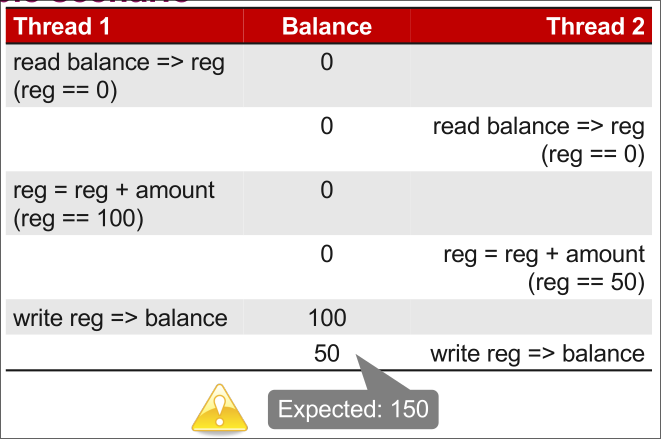
\includegraphics[scale=0.3]{2023_02_27_08_31_29.png}
}[0.6,0.4]

\subsection{Critical Section}
This is a certain part of a job that must be done in sequence, for example a \emph{transaction of a bank}.\newline
\textcolor{purple}{The solution might seem easy, why not just create a locked variable, however, if you do this then you will run into the same problem, When exactly will the lock be written? The same race condition can apply here.} 

\subsection{Synchronized methods in java}
\textcolor{purple}{In java you can mark a method as synchronied to make sure that you will not run into race conditions.}
\begin{lstlisting}
class BankAccount {
  private int balance = 0;
  // function that may not be "truly" multithreaded
  public synchronized void deposit(int amount) {
    this.balance += amount;
  }
}
\end{lstlisting}
\textcolor{purple}{When using these methods, make sure that \emph{ALL} methods that need to be synchronized also have this flag.\newline
In other words if you have a withdraw function and a deposit method, make sure both are marked as synchronized}

\subsubsection{Synchronized Blocks}
You can also just specify a block to be synchronized.\newline
\textcolor{purple}{In this case you need to pass a class to be locked!}
\begin{lstlisting}
class BankAccount {
  private int balance = 0;
  public void deposit(int amount) {
    synchronized(this) {
      // specify the this object to be locked
      this.balance += amount;
    }
    System.out.println("Deposit done");
  }
}
\end{lstlisting}
Similar, you can make locks on both \emph{Classes and Objects}. 
\begin{lstlisting}
class Test {
  synchronized void f() { ... } // object lock
  static synchronized void g() { ... } // class lock
}
class Test {
  void f() { // object lock
    synchronized(this) { ... }
  }
  static void g() { // class lock
    synchronized(Test.class) { ... }
  }
}
\end{lstlisting}

\subsubsection{Multiple locks}
\textcolor{purple}{When a method is recursive and synchronized, the method will have multiple locks, of these, it needs to release all of them at the end for the next thread to aquire the locks.}\newline
In other words, the locks are like refcounting. 
\begin{lstlisting}
synchronized void limitedDeposit(int amount) {
  if (amount + balance <= limit) {
    deposit(amount);
  }
}
synchronized void deposit(int amount) { ... }
// will free the locks once all of the calls are done.
\end{lstlisting}

\subsubsection{wait()}
\textcolor{purple}{The wait method will release the lock and regain it after the thread has received a \emph{wake up call}.}
\begin{lstlisting}
class BankAccount {
  private int balance = 0;
  public synchronized void withdraw(int amount) throws InterruptedException {
    while (amount > balance) {
      wait(); // release lock and go into waiting mode
    }
    balance -= amount;
  }
}
public synchronized void deposit(int amount) {
  balance += amount;
  notifyAll(); // wakeup all waiting threads!
}
\end{lstlisting}
\textcolor{purple}{As you can see, if a thread goes into waiting mode and does not receive a wakeup call, it will not start again.\newline
This can cause \emph{deadlocks}, as you might have multiple threads waiting for something to happen, but nothing ever will.}
\begin{itemize}
  \item \textcolor{orange}{notifyAll} wakes up \emph{all} waiting threads \emph{in the inner waiting room}
  \item \textcolor{orange}{notify} wakes up \emph{a random waiting thread} which is in the \emph{inner waiting room}\newline
\end{itemize} 
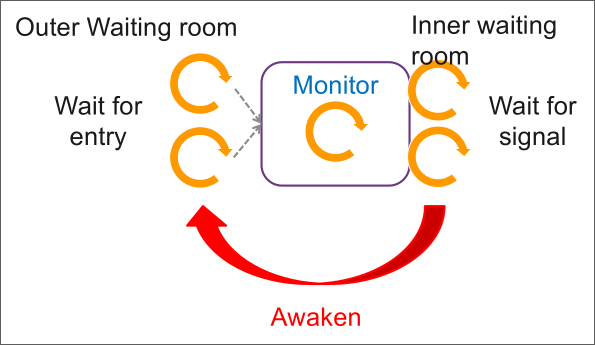
\includegraphics[scale=0.4]{2023_02_27_09_36_15.png}
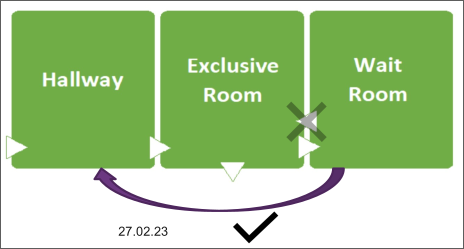
\includegraphics[scale=0.4]{2023_02_27_09_37_23.png}
In other words, wait() will put the thread in the hallway, the operating system will then put the thread into the exclusive room after it is scheduled. From here it can be awoken early with \emph{notifyALL}, or it can wait until it is in the proper waiting room, where it can be called with \emph{notify()}.

\subsubsection{Traps with Monitors}
\textcolor{purple}{Trap 1: IF}
\begin{lstlisting}
public synchronized void put(T x) throws InterruptedException {
  if (queue.size() == capacity) {
    wait(); // await non-full
  } // oops we only waited once, if the capacity is still to small we now have a problem!
  queue.add(x);
  notify(); // signal non-empty
}
// instead!
while (!condition) {
  wait(); // this makes sure that we will wait even after the thread gets another lock!
}
\end{lstlisting}
\textcolor{purple}{Trap 2: Overtaking}\newline
\textcolor{teal}{Here the issue is that if you use notify(), you are going to call a random thread, in case you need serialization, you will not be achieving this with notify(), \emph{instead use notifyALL()!}}
\begin{lstlisting}
// ...
queue.add(x);
notify(); // signal non-empty
\end{lstlisting}
\textcolor{purple}{Trap 3: Eternal Wait}\newline
\textcolor{teal}{Here the issue is that with a single notify(), you might awaken a thread that will then also wait for another condition, which will not notify any other thread, meaning that there is no further notify chaining.\newline
You will now wait for something that will never be done, good job :)}

\subsection{Spurious Wake-up}
\textcolor{purple}{This is a OS specific feature, for example for POSIX operating systems.}\newline
Here the thread can \emph{spuriously awaken without a specific notify}, this is something that you as a developer have to guard against!

\subsection{When a single notify is enough}
\begin{lstlisting}
public class Turnstile {
  private boolean open = false;
  public synchronized void pass()
  throws InterruptedException {
    while (!open) { wait(); }
    open = false;
  }
  public synchronized void open() {
    open = true;
    notify(); // or notifyAll() ?
  }
}
\end{lstlisting}
\textcolor{purple}{Here the idea is that if one passes, only one new thread can be reactivated. 1 in, 1 out.\newline
This means that you can't notify everyone -> would unnecessarily wake up other threads.}\newline
\textcolor{teal}{The other condition that needs to be true is that every waiting thread is waiting for the same condition!} 
\begin{itemize}
\item \textcolor{teal}{1 in, 1 out}
\item \textcolor{teal}{same condition for every thread}
\end{itemize} 

\subsection{Fairness}
\textcolor{purple}{When calling notify, we have no guarantee of order which thread will be woken up. This is called the problem of \emph{fairness}.\newline
notifyAll \emph{helps this by waking up EVERY thread.}}\newline
\textcolor{red}{In short, with java monitor, you either have the \emph{fairness problem with notify}, or \emph{inefficiency with notifyAll}!}

\section{Synchronization Methods}

\subsection{Semaphore}
\begin{itemize}
\item \textcolor{purple}{Essentially a counter for resources}
\item \textcolor{purple}{acquiring resource -> -1}
\item \textcolor{purple}{releasing resource -> +1}
\item \textcolor{purple}{wait for resource if necessary}
\item \textcolor{purple}{relatively low level and efficient! -> no notifyAll!!}
\end{itemize} 

\subsubsection{Semaphore in java, geil}
\begin{itemize}
\item \textcolor{purple}{acquire() => P()}\newline
  if not available, wait until another thread releases
\item \textcolor{purple}{release() => V()}\newline
  \textcolor{red}{You can always call release! This means you can create fake resources, it is your responsibility to make sure to not call release in this case!}
\end{itemize} 
\begin{lstlisting}
public class Semaphore {
  private int value;
  public Semaphore(int initial) {
    value = initial;
  }
  public synchronized void acquire() throws InterruptedException {
    while (value <= 0) { wait(); }
    value--;
  }
  public synchronized void release() {
    value++;
    notify();
    here
  }
}
\end{lstlisting}

\subsubsection{Types of semaphores}
\begin{itemize}
\item \textcolor{purple}{General Semaphore -> from 0 to N}\newline
  \begin{itemize}
  \item \textcolor{black}{new Semaphore(N)}
  \item \textcolor{black}{Up to N threads are allowed to acquire at the same time.}
  \item \textcolor{black}{for limited resources/quotas etc}
  \end{itemize} 
\item \textcolor{purple}{Binary Semaphore -> 0 or 1}\newline
  \begin{itemize}
  \item \textcolor{black}{new Semaphore(1)}
  \item \textcolor{black}{For mutual exclusion (1 = open, 0 = closed)}
  \end{itemize} 
\item \textcolor{purple}{Fair Semaphore}\newline
  \begin{itemize}
  \item \textcolor{black}{New Semaphore(N, true)}
  \item \textcolor{black}{uses FIFO for fairness}
  \item \textcolor{black}{the longest waiting thread gets resource}
  \item \textcolor{black}{slower than other variants}
  \item the true or false flag defines if the semaphore is fair -> flag
  \end{itemize} 
\end{itemize} 

\subsection{Bounded Buffer with Semaphores}
\begin{lstlisting}
class BoundedBuffer<T> {
  private Queue<T> queue = new LinkedList<>();
  private Semaphore upperLimit = new Semaphore(Capacity, true); // lowerbound of buffer
  private Semaphore lowerLimit = new Semaphore(0, true);        // upperbound of buffer
  private Semaphore mutex = new Semaphore(1, true);             // mutex to ensure no race conditions
  public void put(T item) throws InterruptedException {
    upperLimit.acquire();
    mutex.acquire(); queue.add(item); mutex.release();
    lowerLimit.release();
  }
  public T get() throws InterruptedException {
    lowerLimit.acquire();
    mutex.acquire(); T item = queue.remove(); mutex.release();
    upperLimit.release();
    return item;
  }
}
\end{lstlisting}

\subsubsection{Multi release/acquire}
\textcolor{purple}{You can release or acquire multiple resources at once with \emph{release(n) or acquire(n)}, with n being a random number.}

\section{Lock conditions}
Before we only worked with one monitor, however that is not always ideal. Usually we want to work with many waiting rooms, monitors etc.\newline
In this case using synchronized can be very harsh on performance, instead we can use \emph{multiple waiting rooms and locks.} 
\begin{lstlisting}
Lock monitor = new ReentrantLock(true);
Condition nonFull = monitor.newCondition();
Condition nonEmpty = monitor.newCondition();
\end{lstlisting}
\textcolor{purple}{Here we have a nonFull queue and a nonEmpty queue, as well as a lock to ensure no race conditions! -> mutex}\newline
Here is how you would then go ahead to use this: \newline
\begin{lstlisting}
class BoundedBuffer<T> {
  private Queue<T> queue = new LinkedList<>();
  private Lock monitor = new ReentrantLock(true);
  private Condition nonFull = monitor.newCondition();
  private Condition nonEmpty = monitor.newCondition();
  public void put(T item) throws InterruptedException {
    monitor.lock();
    try {
      while (queue.size() == Capacity) { nonFull.await(); }
      queue.add(item);
      nonEmpty.signal(); Loop to avoid spurious wakeup
    } finally { 
    monitor.unlock();
    }
  }
  public T get() throws InterruptedException {
    monitor.lock();
    try {
      while (queue.size() == 0) { 
      nonEmpty.await();
      }
      T item = queue.remove();
      nonFull.signal();
      return item;
    } finally { 
      monitor.unlock(); 
    }
  }
}
\end{lstlisting}

\subsubsection{Methods}
\begin{itemize}
\item \textcolor{purple}{room.signal() -> same as notify()}
\item \textcolor{purple}{room.signalAll() -> same as notifyAll()}
\item \textcolor{purple}{room.await() -> same as wait()}\newline
  Just like wait() room.await() throws that annoying exception...
\item \textcolor{purple}{lock()/unlock() -> same as synchronized blocks}
\end{itemize} 

\subsection{Read-Write Locks}
\textcolor{purple}{Just like rust does by default, the idea is that you can read as long as you don't write, meaning you can either have \emph{unlimited reads OR one write}.}

\subsection{Countdown Latch}
\textcolor{purple}{This is simply condition where you would need \emph{more than 1 thread to be done with their execution}. \newline
For example, in order for an F1 race to be over, you need all cars over the line. This can easily be done \emph{by using a counter}, each car will decrement the counter, and the race is over when the count is 0.}\newline
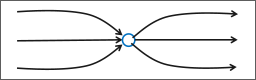
\includegraphics[scale=0.4]{2023_03_06_09_43_52.png}

\subsection{Cyclic Barrier}
\textcolor{purple}{This is essentially a \emph{reusable countdown latch}, when the count is 0 at the end of the race, it will be reset for the new race.}\newline
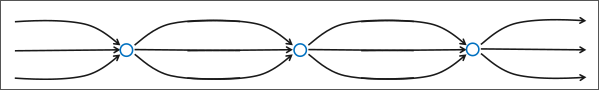
\includegraphics[scale=0.4]{2023_03_06_09_44_14.png}

\subsection{Exchanger}
\textcolor{purple}{When \emph{2 threads} stop simultaneously, they can exchange information. If one thread calls exchange, it is blocked until the other thread also calls exchange.}\newline
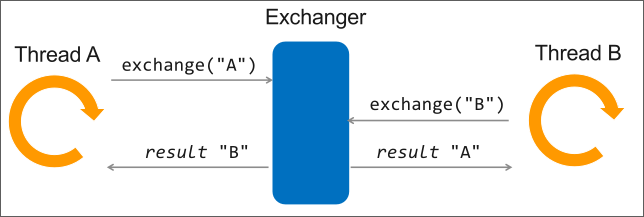
\includegraphics[scale=0.4]{2023_03_06_09_47_31.png}\newline
\textcolor{red}{Example:}
\begin{lstlisting}
var exchanger = new Exchanger<Integer>();
for (int count = 0; count < 2; count++) {
  new Thread(() -> {
    for (int in = 0; in < 5; in++) {
      try {
        int out = exchanger.exchange(in);
        System.out.println(
        Thread.currentThread().getName() + " got " + out);
      } catch (InterruptedException e) { }
    }
  }).start();
}
\end{lstlisting}

\section{Problems with concurrency}

\subsection{Race Conditions}
This is nondeterministic behavior. \newline
Eg. wrong order of execution -> addition before multiplication.\newline
This can occur with, OR without data races.\newline
An example of a race condition even with synchronized is this:
\begin{lstlisting}
class BankAccount {
int balance = 0;
synchronized int getBalance() { return balance; }
synchronized void setBalance(int x) { balance = x; }
} // problem: we can use getBalance and setBalance in the wrong order, even though
// the updates themselves are now protected, meaning there is no write or read at the same time! 
// Rust also can't solve this issue, this is a programmer issue!!
\end{lstlisting}

\subsubsection{Data Races}
Eg. two threads that want to access the same variable/object at the same time.\newline
In this case there is no method that guarantees any sort of serialization, instead it is random.\newline
\textcolor{teal}{Note, for a data race to occur, there needs to be \emph{at least one write access with either one or more additional write OR read access}, \newline
this is exactly what the rust borrow checker enforces!}\newline

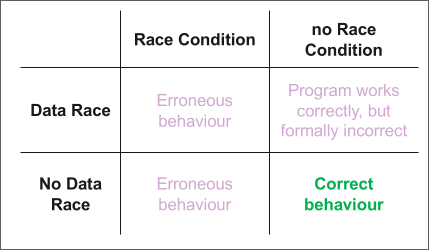
\includegraphics[scale=0.4]{2023_03_13_08_42_17.png}

\subsection{Confinement / Thread Safety}
This limits the availability of objects/variables to something specific, eg. specific thread, or only inside synchronized functions/objects.\newline
\textcolor{teal}{Thread safety simply means the elimination of data races. Note, race conditions can still occur!}

\subsubsection{Thread Confinement}
This ensures that the object is only accessible via a reference of a specific thread.

\subsubsection{Object Confinement}
This ensures that the object is only accessible inside of other synchronized objects.
\begin{lstlisting}
class ProductDatabase {
  private final HashMap<String, Product> productMap = new HashMap<>();
  public synchronized void addProduct(String name, String details) {
    productMap.put(name, new Product(details));
  }
  public synchronized String getProductDetails(String name) {
    return productMap.get(name).getDetails();
  }
  public synchronized void notifySale(String name) {
    productMap.get(name).increaseSales();
  }
}
\end{lstlisting}

\subsection{Thread Safety and Jafuck collections}
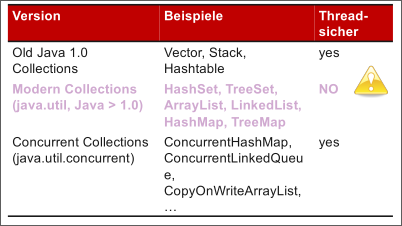
\includegraphics[scale=0.4]{2023_03_13_09_09_23.png}\newline
\textcolor{teal}{In general, you always need to make sure that everything you use is thread safe, in general, older collections are thread safe with more modern ones not being thread safe for some reason.\newline
Probably because jafuck is a horrible language and no longer has any right to exist.}

\subsection{Deadlocks}
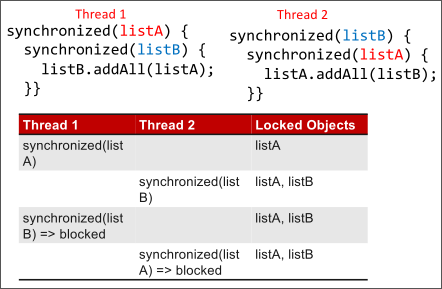
\includegraphics[scale=0.4]{2023_03_13_09_17_53.png}\newline
Deadlocks can also happen with synchronized, as the thread itself will be locked when used: 
\begin{lstlisting}
class BankAccount {
  private int balance;
  public synchronized void transfer(BankAccount
  to, int amount) {
    balance -= amount;
    to.deposit(amount);
  }
  public synchronized void deposit(int amount) {
    balance += amount;
  }
}
a.transfer(b, 20); // acquires lock to b
b.transfer(a, 50); // oops....
\end{lstlisting}

\subsubsection{Live Locks}
\textcolor{red}{This is a special case of deadlocks, where the cpu is actually still working, eg. it is in a while loop waiting for a lock to be released.\newline
However, that lock will never be released, as two threads have blocked each other!}\newline
This is even worse than deadlocks, as this means the cpu will waste power on garbage.

\subsubsection{Dealing with Deadlocks}
\textcolor{teal}{You could lock linearly, meaning that you will start with 1 lock and expand as needed.\newline
Other threads can't start locking, as the base is already locked. \newline
Note that depending on how deep the base lock is, you can call it a "granular lock" -> lock at root}\newline
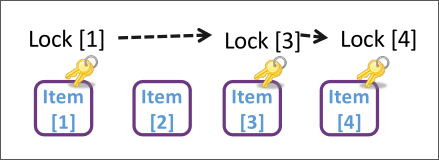
\includegraphics[scale=0.4]{2023_03_13_09_34_03.png}
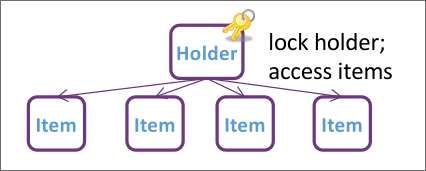
\includegraphics[scale=0.4]{2023_03_13_09_35_29.png}

\subsection{Starvation}
\textcolor{red}{This happens when the lock avoidance leads to certain threads not being able to do their job. \newline
Eg the submissive thread that always releases its lock as soon as someone else wants it will never actually be able to finish its task, meaning that you might end up with a problematic state that blocks or even crashes your program.}\newline
\textcolor{teal}{The best way to deal with this is using something like semaphores that will enforce fairness, but always keep in mind that this will be \emph{at the cost of performance.}}

\subsection{Parallelism}
In the end what we want is a program that has \emph{no race conditions, no deadlocks and no starvation, with still decent performance.}

\section{C\#}../ost-summary-template.tex

\subsection{Basics}

\subsubsection{Spawning Threads}
\begin{lstlisting}
var myThread = new Thread(() => {
  for (int i = 0; i < 100; i++) {
    Console.WriteLine("MyThread step {0}", i);
  }
});
myThread.Start();
myThread.Join();
\end{lstlisting}

\subsubsection{Monitor in C\#}
\begin{lstlisting}
class BankAccount {
  private decimal balance;
  public void Withdraw(decimal amount) {
    lock (syncObject) {
      while (amount > balance) {
        Monitor.Wait(syncObject);
      }
      balance -= amount;
    }
  }
  public void Deposit(decimal amount) {
    lock (syncObject) {
      balance += amount;
      Monitor.PulseAll(syncObject);
    }
  }
}
\end{lstlisting}

\section{Thread Pools}

\subsection{Problem with Threads}
\begin{itemize}
\item \textcolor{teal}{scheduling needs time }
\item \textcolor{teal}{thread might awake only for it to wait again since condition is not met}
\item \textcolor{teal}{limited in numbers}
\item \textcolor{teal}{every thread needs a stack for itself}
\item \textcolor{teal}{preemptive full register-backup for each thread}
\end{itemize} 

\subsection{Solution}
Instead of using \emph{all threads all the time}, we only use some of them. (at least as many as physical cores)\newline
\textcolor{teal}{Then we define the functionality in question as \emph{task} instead.\newline
These tasks can then be parallelized, or not, depending on the functionality in question.}

\subsection{Task Queue}
Tasks are handled as a queue, from which threads can take individual tasks from.\newline
The thread will then execute said task and proceeds to take a new one.\newline
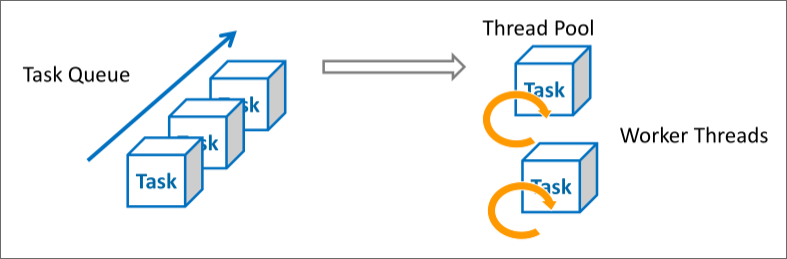
\includegraphics[scale=0.4]{2023_03_20_08_25_48.png}\newline
Benefits:
\begin{itemize}
\item \textcolor{green}{scalable -> more threads or cores automatically means more performance}
\item \textcolor{green}{easily made to run in parallel -> multi CPU structures}
\end{itemize} 

\subsubsection{Run To Completion}
As already stated above, each task needs to be run to completion, however \emph{this does not apply to nested subtasks}, \newline
this is because you might encounter deadlocks with other tasks if you would want to guarantee this as well.\newline
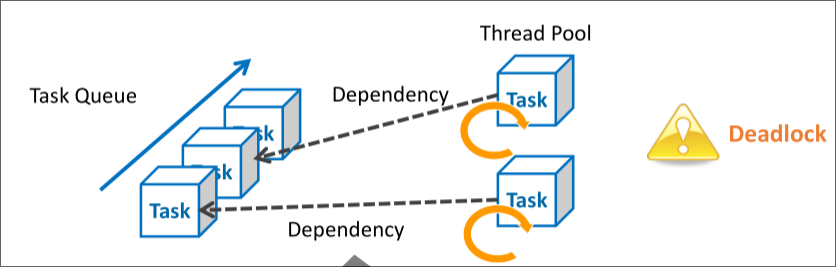
\includegraphics[scale=0.4]{2023_03_20_08_29_42.png}

\subsection{Thread Pools in Java}
\begin{lstlisting}
var threadPool = new ForkJoinPool();
Future<Integer> future = threadPool.submit(() -> {
  // this is the task to execute
  int value = 50;
  // do something with value
  return value;
});
\end{lstlisting}
\textcolor{teal}{Essentially a promise in js, you don't know if it is done or not.\newline
To check use the following:}
\begin{lstlisting}
Future<T> future = threadPool.submit(yourtask); // launch task
T result = future.get(); // blocks until result is here
\end{lstlisting}
\textcolor{red}{Note, unlike js, the get() function will \emph{block the thread} until the result is here!!}

\subsubsection{Thread Pool Instantiation}
\begin{lstlisting}
// explicit pool
var threadPool = new ForkJoinPool();
int result = threadPool.invoke(new CountTask(2, N));

// using default pool
int result = new CountTask(2, N).invoke();
\end{lstlisting}
\textcolor{teal}{Important, when using the default pool, it will not always use all processors, as it does internal optimization.}

\subsubsection{Functions}
\begin{itemize}
\item \textcolor{purple}{RecursiveAction}\newline
  like RecursiveTask<Void> -> simply no return value
\item \textcolor{purple}{invokeAll()}\newline
  start and wait for sub-tasks -> invokeAll(task1, task2)
\item \textcolor{purple}{submit()}\newline
  create a new task
\item \textcolor{purple}{get()}\newline
  block until result is here
\item \textcolor{purple}{invoke()}\newline
  run task
\item \textcolor{purple}{cancel()}\newline
  cancel task
\item \textcolor{purple}{fork()}\newline
  split task into subtasks 
\item \textcolor{purple}{join()}
  wait for the other task to finish after own execution has stopped
\end{itemize} 

\subsubsection{Parallel Counting Example}
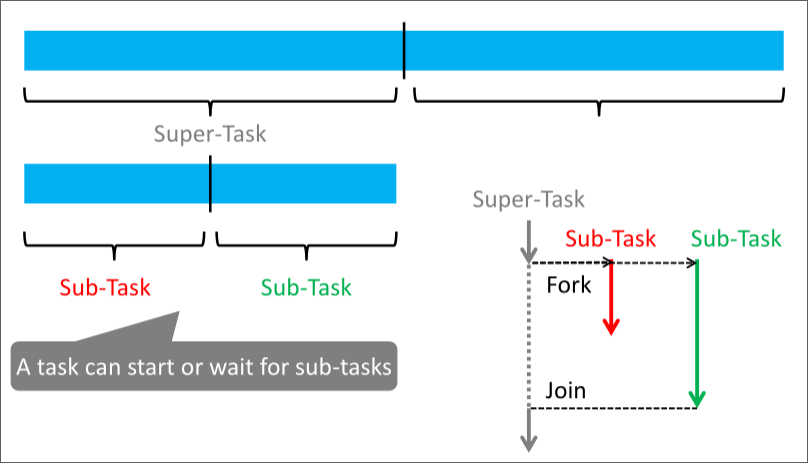
\includegraphics[scale=0.4]{2023_03_20_08_40_04.png}
\begin{lstlisting}
class CountTask extends RecursiveTask<Integer> {
  // Constructor
  @Override
  protected Integer compute() {
    // if no or single element => return result
    // split into two parts
    var left = new CountTask(lower, middle);
    var right = new CountTask(middle, upper);
    left.fork(); right.fork();
    return right.join() + left.join();
  }
}
\end{lstlisting}

\subsubsection{Full Task Implementation}
\begin{lstlisting}
class CountTask extends RecursiveTask<Integer> {
  private final int lower, upper;
  public CountTask(int lower, int upper) {
    this.lower = lower; this.upper = upper;
  }
  protected Integer compute() {
    if (upper - lower > THRESHOLD) {
      // parallel count
      int middle = (lower + upper) / 2;
      var left = new CountTask(lower, middle);
      var right = new CountTask(middle, upper);
      left.fork(); right.fork();
      return right.join() + left.join();
    } else {
      // sequential count
      int count = 0;
      for (int number = lower; number < upper; number++) {
      if (isPrime(number)) { count++; }
    }
    return count;
  }
}
\end{lstlisting}

\lstset{
    language=C#,
    style=code,
}

\subsection{Thread Pools in C\#}
\begin{itemize}
\item \textcolor{purple}{efficient thread pool by default}
\item \textcolor{purple}{Task Parallization: use tasks explicitly}
\item \textcolor{purple}{Data Parallization: use parallel statements and queries using tasks explicitly}
\item \textcolor{purple}{Asynchronous Programming}
\end{itemize} 
\subsubsection{Tasks in C\#}
\begin{lstlisting}
Task task = Task.Run(() => {
  // task implementation
});
// perform other activity
task.Wait(); // blocking just like in jafuck
\end{lstlisting}

\subsubsection{Task with return Value}
\begin{lstlisting}
Task<int> task = Task.Run(() => {
  int total = … // some calculation
return total;
});
// no wait/get etc necessary!
Console.Write(task.Result); // result of task
\end{lstlisting}

\subsubsection{Nested Tasks}
\begin{lstlisting}
var task = Task.Run(() => {
  // unlike java you don't have to specifically say that you want to wait for the task
  // instead you can just use it in the return.
  var left = Task.Run(() => Count(leftPart));
  var right = Task.Run(() => Count(rightPart));
  return left.Result + right.Result;
});
static Task<int> Count(part) { 
  // do something
}
\end{lstlisting}

\subsubsection{Parallelism without explicit tasks}
Some things can be done in parallel without specifying it. 
\begin{lstlisting}
void MergeSort(l, r) {
  long m = (l + r)/2;
  MergeSort(l, m);
  MergeSort(m, r);
  Merge(l, m, r);
}

void Convert(IList list) {
  foreach (File file in list) {
    Convert(file);
  }
}
\end{lstlisting}

\subsubsection{Parallelism with explicit tasks}
\begin{lstlisting}
Parallel.Invoke(
  () => MergeSort(l, m),
  () => MergeSort(m, r)
);
\end{lstlisting}
\textcolor{red}{Here the continuation is blocked until \emph{both threads have stopped executing!}}

\subsubsection{Data Parallel ForEach}
\begin{lstlisting}
Parallel.ForEach(list,
  file => Convert(file)
);
\end{lstlisting}
\textcolor{red}{Queue a task for each item in the foreach sequence. This blocks by default until all taks are done!}

\subsubsection{Data Parallel For}
\begin{lstlisting}
for (i = 0; i < array.Length; i++) {
  DoComputation(array[i]);
} // sequential
Parallel.For(0, array.Length,
  i => DoComputation(array[i])
); // parallel, only works in case iterations are independent!
\end{lstlisting}
\textcolor{red}{Please note, for the second variant the iterations need to be independent.}

\subsubsection{Parallel Loop Partitioning}
When you iterate through an array, you might want to split the iterations to multiple threads.\newline
However, making each iteration run on a new thread is really inefficient, so what can we do?\newline
\textcolor{teal}{We split based on algorithms:}\newline
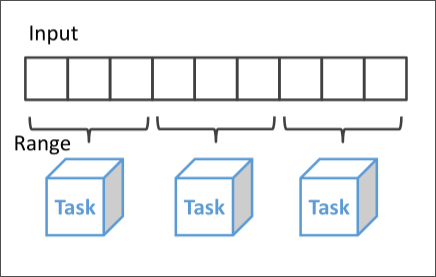
\includegraphics[scale=0.4]{2023_03_20_09_23_13.png}\newline
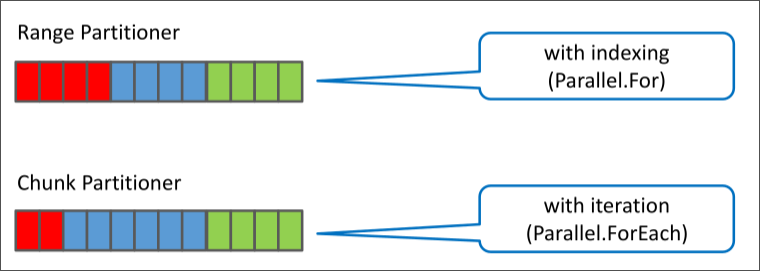
\includegraphics[scale=0.4]{2023_03_20_09_24_26.png}\newline

\subsubsection{Parallel For with Thread-Local Variables}
\begin{lstlisting}
long total = 0;
Parallel.For<long>(
  0, array.Length,
  () => 0,
  (i, _, subtotal) => {
    subtotal += array[i];
    return subtotal;
  },
  subtotal => Interlocked.Add(ref total, subtotal)
);
\end{lstlisting}

\subsubsection{Parallel LinQ}
\begin{itemize}
\item \textcolor{purple}{Parallelization of language-integrated query (sql like)}
\item \textcolor{purple}{Data Parallelism}
\item \textcolor{purple}{Similar to Java Stream API}
\end{itemize} 
Examples: 
\begin{lstlisting}
// Get ISBN of all books with the title "Concurrency"
bookCollection
.Where(book => book.Title.Contains("Concurrency"))
.Select(book => book.ISBN)

// Map each number in a list to a bool value (true = prime number)
inputList
.Select(number => IsPrime(number))
\end{lstlisting}
You can also make this work with a sql like query 
\begin{lstlisting}
// Get ISBN of all books with title "Concurrency"
from book in bookCollection
where book.Title.Contains("Concurrency")
select book.ISBN

// Map each number in a list to a bool value (true = prime number)
from number in inputList
select IsPrime(number)
\end{lstlisting}
If you want to use this with \emph{parallelization}: 
\begin{lstlisting}
// Get ISBN of all books with title "Concurrency"
from book in bookCollection.AsParallel()
where book.Title.Contains("Concurrency")
select book.ISBN
Results in random order

// Map each number in a list to a bool value (true = prime number)
from number in inputList.AsParallel().AsOrdered()
select IsPrime(number)
// as ordered makes sure it is still serialized! Otherwise the return order is weird
\end{lstlisting}

\lstset{
    language=Java,
    style=code,
}

\subsubsection{Comparison to Java Stream API}
\begin{lstlisting}
// Get ISBN of all books with title "Concurrency"
// Allow unordered explicitly (by default ordered in java)
bookCollection.parallelStream().unordered()
.filter(book -> book.getTitle().contains("Concurrency"))
.map(book -> book.getISBN());

// Map each number in a list to a bool value (true = prime number)
inputList.parallelStream()
.map(number -> isPrime(number));
\end{lstlisting}

\lstset{
    language=C#,
    style=code,
}

\subsubsection{Work Stealing Thread Pool}
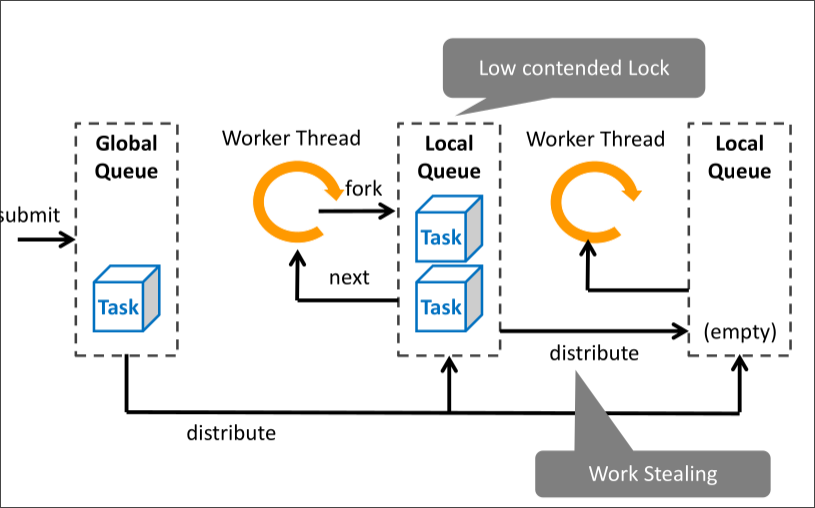
\includegraphics[scale=0.4]{2023_03_20_09_32_19.png}\newline
A thread will take multiple tasks from the global pool and then start working on them.\newline
Should one thread be done with all tasks and there is still work to be done on other threads, the now afk thread will steal a task from the other threads.

\subsubsection{Thread Injection}
\textcolor{teal}{This is the idea that a controller will automatically add threads to certain tasks (\emph{at runtime!}) if it sees a benefit in terms of runtime.\newline
It does this with a \emph{Hill Climbing Algorithm}, by measuring throughput}. \newline
In general this does solve deadlocks, but it is slower than regular thread pools. (deadlocks still possible with ThreadPool.SetMaxThreads())

\end{document}
